\documentclass{article}
\usepackage[utf8]{inputenc}
\usepackage{graphicx}
\usepackage{fancyvrb}
\graphicspath{{./images}}

\title{COS30031 Games Programming\\Custom Project Report}
\author{Daniel Coady 102084174}
\date{17/11/2021}

\begin{document}

\maketitle

\pagebreak

\tableofcontents

\pagebreak

\section{Introduction}
\subsection{Background}
Computers are incredible and complicated these days, with many components that
allow for the more efficient and effective computation of various tasks. For me
personally, by far the most interesting modern day development (which many will
actually take for granted) is the humble GPU. Short for graphics processing
unit, it is a core aspect to any computer whether it is pushing hyper-realistic
game graphics or displaying the words on your social media feeds. These GPUs
differ greatly from the CPU which many view as the beating heart of any
computer. CPUs have been designed to be more general purpose, allowing for
operations such as logical branching, maths, and bitwise magic. GPUs on the
other hand are entirely focused on floating point maths operations, and have
been architected to be able to do those rapidly and in parallel. This means
modern day graphics requirements, such as being able to independently address
one of the literal millions of pixels on your screen (a standard 1080p screen
contains a little over 2 million pixels!), is now a trivial task that can be
completed with great speed.

Computers haven't always been like this however, and many moons ago we would
have required the CPU to perform all of the logical and graphical work of a
computer. This complicated matters greatly as soon as you wanted to display
complex graphics, and it only got worse if you wanted to display complex
graphics \textit{and} provide complex logic--such as in a game. It's for this
reason that many games of yore have had to come up with some very clever
techniques to "cheat" graphics. Most games for the longest time were purely 2D
since that was about as much as we could reasonably handle with the hardware
at the time. Before 3D accelerated technology hit the general consumer market,
3D games were but a dream... Kind of.

Enter the raycaster. There will be more later on about how it works and why it's
so fast, but for now just know that raycasters were some of the earliest
attempts at creating 3D graphics in games. Not to be confused with ray marching
and ray tracing (two very cool 3D graphics techniques as well!), raycasters have
a very distinct look to them that many will remember from the first Wolfenstein
3D game. They tend to look very blocky, with billboarded sprites representing
the entities within a scene. This technology forms the basis of my custom
project.

\subsection{The Project}
At a high level, this project will take form of a first person shooter using
3D raycaster graphics. The front end will use SFML to display the internal frame
buffer as well as receive/process the window events. The back end will be far
more complex, consisting of the actual raycasting engine, an ECS implementation
for managing enemy entities, multi-threading to assist with performance, and
some simple collision detection. The entire project has been written in C++
within a Linux environment using the gcc toolchain, and borrows greatly both
from Austin Morlan's writeup on ECS\footnote{https://austinmorlan.com/posts/entity\_component\_system/}
and Dmitry V. Sokolov's tinyraycaster series of tutorials\footnote{https://github.com/ssloy/tinyraycaster/wiki/Part-0:-getting-started}.
All code for this project will be available on GitHub\footnote{https://github.com/pondodev/custom-project}
under the Unlicense License.

\section{Implementation}

\subsection{Front End}
The bulk of the front end in this project is handled by the Simple and Fast
Multimedia Library, or SFML for short. SFML is similar to SDL in a variety of
ways--both have many useful abstractions of low level graphics, image handling,
audio processing, etc. There are some key differences between the two however:

\begin{itemize}
    \item SDL has a very C style design and API, while SFML's design and API are
          much more like C++
    \item SFML's abstractions tend to be easier to work with due to it's object
          oriented nature
    \item SDL's graphics abstractions are fairly limited, only allowing for
          simple quads and textures while SFML has more primitives and a simple
          shader pipeline
    \item SFML just generally has less boilerplate code than SDL
\end{itemize}

All of the above ultimately influenced my decision to choose SFML over SDL as
we had been using for all of our previous tasks throughout the unit. Add to this
that it has a very sensible system for event polling that is similar (though in
my opinion, slightly better) to SDL's own event system, and it just made sense
for the purposes of my project.

There is another option however, one that I think might have made more sense for
this project: raw OpenGL. It's a scary prospect, for sure, but there's a big
benefit in the form of performance that we would have gained. There is of course
some added complexity that would come from this since we're essentially working
with little to no abstractions. However, considering that there isn't much we
need from SFML outside of the events system and drawing textures to a quad, it
would have been decently trivial to make the change over to raw OpenGL.

\subsection{Back End}

\subsubsection{Enemy AI}
Enemies are all treated as entities in an Entity Component System, or ECS for
short. This is quite a simplified version of ECS, as it only need serve one
specific purpose with little to no generics involved. This has allowed me to
keep it as simple as it is, while also ensuring maximum performance from both
algorithmic and cache optimisations.

Each entity will contain a component for movement, the enemy type, and the
distance it is from the player. They have been separated like this since there
are situations where not all of the data related to an entity would be
necessary, and so by lowering the amount of data we need to retrieve in each of
the related systems we can help ensure higher amounts of data are being fetched.
In terms of systems present, there are a few present. The main ones are the
render system, and the enemy behaviour system. The render system is fairly
uninteresting as all it does is read the components for each entity to render
them accordingly. The enemy behaviour system on the other hand is far, far more
interesting. This system, as the name would imply, is where all of the actual
AI for each enemy lives. The enemy AI is incredibly simple, as it exhibits only
two behaviours: chasing the player and waiting to see the player.

Chasing the player is fairly simple: calculate the unit vector pointing towards
the player, then add that vector to the current position scaling by speed and
current delta time. This only happens when the enemy can see the player however,
and this was a fair bit more complex. You see, physics raycasting with my
current solution is rather complicated due to there being no real collision
detection to speak of. If I had implemented some simple collision detection with
axis-aligned bounding boxes then I may have been able to do some simple maths to
check for ray intersections with edges of the AABB, but there is no such thing
implemented. So there's only really one option left for me: a sort of ray march.
To be clear, this isn't the graphics technique for volumetric raycasting, I just
don't have a better name for it at the time of writing this. Simply put, the way
that the physics raycasting works is by continually "marching" in a given
direction until it hits something. If we hit something, then we register what
that is and make a decision based on that. In our case, if we hit a wall then we
don't want to move the entity. If it hits the player, then we start chasing.

This gets expensive to perform every frame however, so I wanted a way to make it
more performant. This posed an interesting issue since more performance seemed
to require me to give up some amount of accuracy. This lead me to perform a
series of tests on how performant and accurate different levels of coarseness
were when performing a physics raycast, but perhaps most importantly I wanted to
find out at what point did the believability of the AI suffer. Much to my
surprise, I could go incredibly coarse before it started to show any sort of
behaviour that was odd. And so, I made the raycast treat each map tile as a
single unit, and it will draw a line from enemy to player checking for a hit.
This hit a good balance, where the entities never ended up showing strange
behaviour, but performance is hardly impacted due to how coarse the physics
raycast calculations are.

\subsubsection{Collision Detection}
Unfortunately, there was not much in the way of physics collision detection
implemented into this project. Much of this comes down to problems with time
constraints, as there has not been enough time to work it in, and the limited
time I have had at my disposal caused me to make some poor decisions when it
came to architecture which ended up not lending itself well to implementing
even simple collision systems.

Bar the previously mentioned physics raycasting for enemy movement, there is one
other area where I have implemented collision detection: player movement.
Well... In theory at least. The idea is that the player shouldn't be able to
walk into walls (both because walls are solid, but also because it crashes the
game) and this is achieved with the following code:

\begin{verbatim}
// in the update method
if ( get_map_tile( int(player.position.x), int(old_pos.y) ) != Floor ) {
    float wall_start = floor( player.position.x );
    if ( move_vec.x < float(0) ) wall_start += 1.0;
    else wall_start -= 0.05;
    player.position.x += wall_start - player.position.x;
}

if ( get_map_tile( int(old_pos.x), int(player.position.y) ) != Floor ) {
    float wall_start = floor( player.position.y );
    if ( move_vec.y < 0 ) wall_start += 1.0;
    else wall_start -= 0.05;
    player.position.y += wall_start - player.position.y;
}
\end{verbatim}

The idea is that when we move, we want to check if there's a wall where we have
just tried to move. If there is, then we move the player back a small amount to
ensure they don't go inside of the wall. Now this actually works excellently,
but only without multi-threading. This is something that I have tried to resolve
and have failed, even with my attempts to ensure that all resources in the hot
path are locked with a mutex. It's really quite strange, but once again due to
time constraints I was unable to do much more with it and had to cut my losses.

\subsubsection{Multi-threading}
Multi-threading is something that you see thrown around a lot as a way to get
free or easy performance. Well, I'm happy to report that those people are big
fat liars. There are many more complications that come along with implementing
multi-threading into any application, and I encountered a fair few of these
while working it into my current solution.

For some context, the goal of this was to completely decouple the front end from
the back end in such a way that they don't rely on each other executing in
sequence. This allows for one or the other to complete their own loops without
being blocked by the other, which is incredibly important for the front end to
ensure that the application always feels responsive. The way that this was
achieved was by first putting both parts of the program onto their own threads
and then analysing what resources were being shared between the two threads.
Anything that was being shared was then given a mutex to lock it so that all
outputs of the code would still remain deterministic.

In theory this should have preserved functionality, and it did for the most
part. However, bugs still worked their way in and due to the nature of
multi-threaded applications, they were incredibly hard to track down and fix.
But that's perhaps not the worst part is that performance didn't get better--it
actually got worse. Herein lies the crux of the problem with multi-threading:
it's absolutely a powerful tool, but not the right choice for every application.
The reason for this is while adding a new thread to your application absolutely
frees up other threads to work, by virtue of how you have to ensure thread
safety you may actually end up with the same issue I have had. This is because
when adding a mutex, there is an associated overhead with managing it. To add
to this, if you're not careful about using it only as needed then you may block
other threads enough to defeat the purpose of the multiple threads. As a final
nail in the coffin, every thread has the problem of overhead. In order to create
and manage a thread there is an amount of memory and CPU time required. If you
cannot offset this overhead with the performance gained from moving
functionality to a new thread, then you're always going to have worse
performance.

So ultimately, the lesson to be learned here is that multi-threading is not a
pancea. One must ensure they properly assess the benefits and drawbacks to
multi-threading their application lest they end up with worse performance and
more bugs than before.

\subsubsection{Raycaster}
Now for the moment (I hope) you've all been waiting for--raycasting! I need to
get this out of the way before I say too much more: I \textit{love} raycasters.
I think they're some of the coolest ways we "hacked" graphics in the days of
yore, and as such you'll probably find me gushing fairly frequently about just
how cool I think they are. Sorry about that in advance.

So I suppose the next thing to explain is what raycasters are, and why they
exist. In simple terms, raycasters are a way for us to cheat perspective to
create 3D-like environments. To explain how it achieves this, we should explore
how graphics works at a high level first.

In modern graphics APIs (such as OpenGL) we have what is called a graphics
pipeline. This pipeline is made up of individual steps that we pass data through
in order to process it into the pretty visuals we see on our screen. Each of
these steps contains discrete programs which we call shaders, and of note to us
is a specific shader called the fragment shader. Once all the processing on
vertices, normals, etc is done by previous shaders we are now ready to render
our fragments. For our purposes you can simply think of a fragment as a pixel on
your screen. Now imagine that for each fragment, we need to perform a
calculation--on a 1920x1080 screen (a standard full HD display resolution) this
means you have to make 2,073,600 calculations. To keep your computer feeling
responsive you need to make sure that these calculations are done multiple times
a second, which could bring up the calculations per second by a factor of 60.
This is a lot of calculations! But our modern PCs with their very, very fancy
GPUs are able to perform many of these calculations in parallel very, very
quickly which allows our CPU to do other stuff while the PC still looks and
feels responsive.

Old PCs weren't like this however. If they did have a GPU, it certainly wasn't
able to perform this many discrete calculations at such a speed as to make true
3D graphics feasible. The raycaster gets around this with a very clever trick:
only perform discrete calculations for every vertical scanline. This means that
on our 1920x1080 screen, instead of you doing some 2 million calculations you
are now only doing 1920--significantly less! So how does it achieve this? Well,
buckle up because there's a fair bit of maths involved. Don't worry though! I'm
really bad at maths so I'll be explaining things in simple terms as much as I
can, since that's how I understand them (at a high level, anyway).

\begin{figure}
\centering
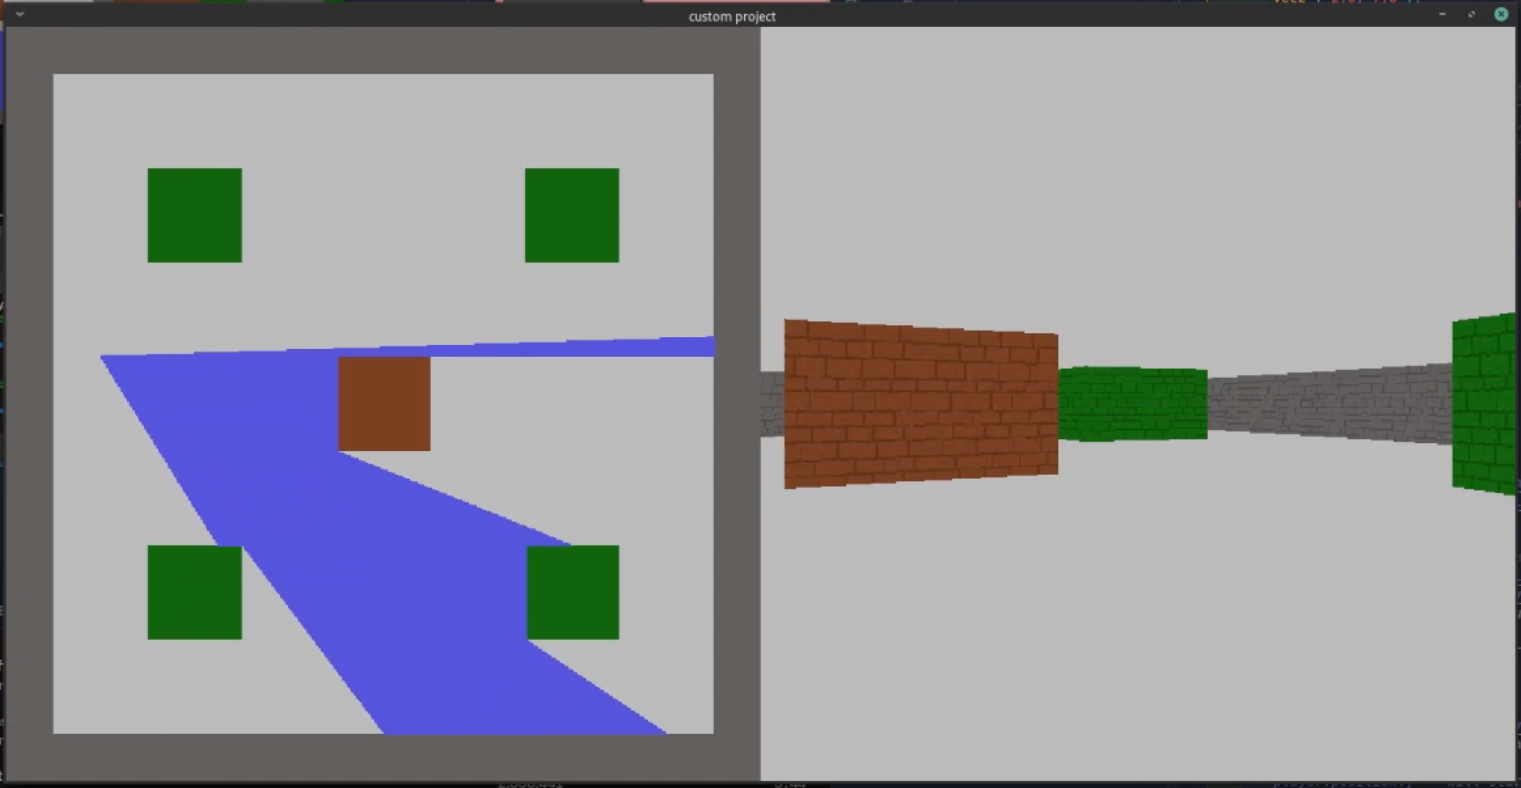
\includegraphics[scale=0.3]{raycaster1.png}
\caption{Demonstration of how the raycaster displays walls in a scene}
\end{figure}

\begin{figure}
\centering
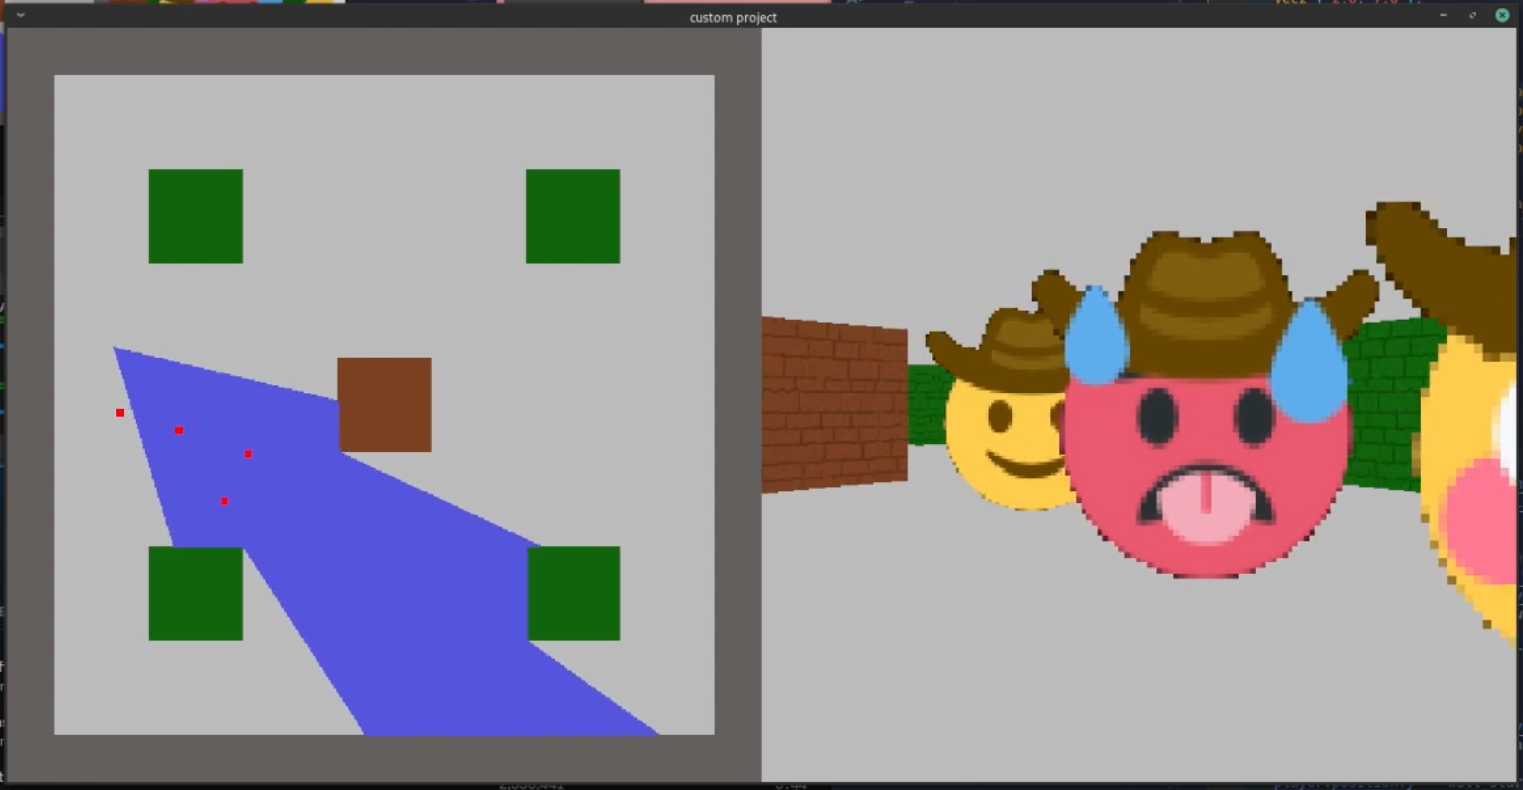
\includegraphics[scale=0.3]{raycaster2.png}
\caption{Demonstration of how the raycaster displays walls and entities in a scene}
\end{figure}

The first thing we start with is the top down 2D projection of the map that we
wish to project with 3D perspective. This becomes our game world, and is
actually what one might consider as the "real" world. This makes operating on
entities in game incredibly easy since they're all entirely within 2D space.
Next we place the player into the world and give them a viewing angle and cone.
This cone will define where all raycasts are made. Now for the magic: we take
the two extremes of the cone and through linear interpolation cast exactly as
many rays as there are pixels horizontally in our render target. For each of
these rays we calculate the distance between the player and the raycast hit.
Depending on how far the hit was, we now draw a vertical bar on the render
target at the appropriate vertical scanline--the closer the hit the larger the
bar, and the further away the hit the smaller the bar. What we've now created
is a really good, simple 3D projection that is incredibly performant and easy to
work with.

Now if we want to add entities to the game, it's more or less the same idea
except now we will be simply calculating the distance between each enemy and the
player. The further away the entity is, the smaller the sprite drawn will end up
being. And that's the bulk of the actual code! There are some more things to it
such as depth testing (which will be talked about later) and lens correction
which I won't really talk about here if only for the sake of brevity, but
suffice to say that this is an incredibly clever and high performance way to
create 3D graphics in games, during a time where such graphics were basically
unheard of.

\section{Challenges}
This has been an absolutely enormous project, one that has spanned months at the
time of writing this. That of course means that there have been many different
and interesting challenges that have arisen during development. I have not
mentioned these challenges above for the sake of brevity, but for the interested
reader I have detailed what they were, why they were problems, and how I did or
didn't manage to resolve them.

\subsection{Raycaster Depth Testing}
Depth testing is a very, very large topic in graphics programming but is still
generally simple enough. The idea is that when we draw something to the screen,
we also want to write a value to the depth buffer. This value is simply how far
whatever was drawn at that pixel is from the camera. What this allows us to do
is perform a depth test on all subsequent draws to see if what we are trying to
draw is in front of or behind something we just drew. This allows us to ensure
that whenever we draw things to the screen, something that is behind another
thing will not get drawn on top.

Since this is a 3D application, there is a simple depth buffer implemented.
Recall that raycasters work entirely on vertical scanlines, which means that our
depth buffer will also work on these vertical scanlines.The process of using
this depth buffer goes as follows:

\begin{itemize}
    \item Draw the walls in the scene, writing it's distance to the depth buffer
    \item Draw each entity in the scene, culling scanlines if a depth test shows it behind a wall
\end{itemize}

This is imperfect as a solution however, and that's because entities may be
drawn on top of each other. You might assume that we can simply write to the
depth buffer as we have already done for the walls, and this does actually work!
But now we have a new kind of issue: transparency. Textures and sprites are not 
columns of a single colour, so when we draw them we need to sample them. Wall
textures are fairly trivial in this regard since we know that they're always
going to be solid with no transparency, so we always draw every pixel of the
texture. Sprites for the entities are a little bit more complicated however, and
this is because they can and do include transparency. Now, the way transparency
is handled in this very simple (in graphics APIs like OpenGL it can get far more
complicated with blend modes and render queues) since all we do is check if
something is transparent at all or not, no translucency is handled. However,
this transparency testing is only done during the sampling of the sprite, there
is no information about it written into the depth buffer.

We could attempt to ensure that all sprites are written to the depth buffer, and
that any transparency is ignored and not written to the depth buffer. This only
works to a point however, because if you recall the depth buffer is only
tracking values for every scanline and there are absolutely cases where a
scanline can be partially transparent. There are many methods to achieve this
kind of depth testing to ensure that sprites are rendered in the correct order,
but I have opted for a brute force method: rendering the entities in ascending
order of distance. This means that the entities which are furthest away from the
player will get rendered first and the closest will be rendered last. This works
simply because anything in front of other entities will just render over it.
It's of course not ideal--we're running a sorting algorithm every frame and
we're wasting resources on rendering more than we can see. A lot of CPU time
gets wasted this way, but it's easy to implement and absolutely works
brilliantly.

\subsection{Mouse Looking}
With the way that the raycaster had been written, changing the player's view
angle would be trivial--and indeed it is. There is a simple method on the Engine
class that allows you to adjust the current player's view angle, which is stored
in radians, by a provided delta. At first this was achieved with a simple button
press which was easy to create: while the key is held down, increment the view
angle by a set delta. This worked excellently, but it would be \textit{way}
cooler if you could control it with your mouse instead.

This is where the complications begin, but not because mouse movements are hard
to track--quite the contrary actually! Really, all that needed to be done was
store the previous position of the mouse, store the next position of the mouse,
and then calculate the magnitude of the two vectors. In fact, this is made even
easier since the only axis we care about is the x axis (raycasters by design
only allow for looking left and right) so we need only store the previous and
current x axis and calculate the difference between the two to get our delta.

In SFML we have, much like SDL does, an event loop. These are pretty simple,
allowing us to listen for all window events. It works incredibly well, and
indeed is perfect for most of what is needed in this project. So when handling a
mouse event, it would seem most reasonable to also add it to this event loop. In
fact, checking the SFML documentation we can see that there is actually an event
type called MouseMoveEvent which is perfect for us. So in theory, we should just
be able to add this event to the loop and calculate our deltas like this:

\begin{verbatim}
sf::Event event;
int last_x;
while ( window->pollEvent( event ) ) {
    // handle other event types here

    switch ( event.type ) {
        case sf::Event::MouseMoveEvent:
            const int delta = event.mouseMove.x - last_x;
            last_x = event.mouseMove.x;
            move_view( delta );
            break;
    }
}
\end{verbatim}

Here is where we encounter our first problem, since if we just calculate the
deltas between the last position and the current position then we may eventually
(and probably will) run out of screen space to travel. To fix this is actually
fairly simple, since we need only do the following:

\begin{verbatim}
// on program init
window->setMouseCursorGrabbed( true );

// during event loop
sf::Mouse::setPosition( window_center, *window );
\end{verbatim}

The general idea is that we are ensuring that the cursor is locked to the window
so we can always capture events, and we're resetting the position to the center
of the window every trip through the loop. This works well, but introduces yet
another issue. You see, when we set the mouse position it actually adds another
MouseMoveEvent to the event stack. This is a problem, because we're in the
middle of polling that very same stack and if we add another event to that stack
while we're in the event loop... Well you're just going to spin endlessly in a
loop--which is exactly what ended up happening.

This problem was the cause for much pain over the course of a few days as I
couldn't figure out how to stop the event stack from registering a new event
when I move the mouse cursor through code. Eventually I happened across a post
on the SFML forums (which unfortunately, I have since lost) which keyed me in to
the solution which I have ultimately landed on. That solution is a simple one:
don't use the event loop. It might be a hack, it might actually be intended,
really I'm not actually sure. What I do know, however, is that calculating the
delta myself outside of the event loop ended up being the solution I needed to
side step the issues with endless looping. However, I do fully admit that
there's a potential issue with performance from this approach (perhaps a small
one, but and issue all the same) since we're still adding these events to the
stack and we're now doing delta calculations on every single frame. These are
sacrifices I'm willing to make however since early optimisation is the enemy of
progress, and there is only so much time to complete this project. Since it
didn't pose any immediate problem with the performance of the project, I've
left it like this in the final product.

\subsection{Shaders}
A big part of why I even looked at SFML in the first place is because of the
shader pipeline--a feature that SDL completely lacked. You see, in graphical
applications there is a need to communicate with graphics APIs such as OpenGL in
order to create all the pretty pictures that you see on your screen. Working
with raw OpenGL is pretty tough though, with much boilerplate needed before you
can even draw a quad. It's why we have high level abstractions over such APIs
like SDL or SFML--they make it significantly easier to create such applications.
However, with abstraction comes a level of control lost, with the big thing
often being granular control over the render pipeline.

In short, a render pipeline is a series of tasks that we complete that will take
in data such as vertices, transform data, normal maps, textures, etc and will
create graphics on your screen. Some of the steps in this pipeline take in code
that will run when data reaches that point of the pipeline, and that code is
called a shader. There are many types of shaders available to a programmer, but
the two main ones that you will see people using are vertex shaders and fragment
shaders. For the sake of brevity I won't dig too deep into what they are (I
leave that as an exercise to the reader!) but just know that they allow us to
perform transforms on individual vertices and create cool visuals using lots of
maths. In fact, anything that you see in games is almost certainly thanks to a
shader doing a lot of heavy lifting.

So as I alluded to before, there's no pipeline exposed to the programmer in SDL
which is a real bummer because I really wanted to mess around with them
(graphics programming is a passing interest of mine that I like to practice
from time to time in my own game dev) and create some neat visual effects. SFML
on the other hand provides a way for you to tap into it's pipeline to insert
your own custom vertex and fragment shaders. This is something I intended to
use to do... Something with. I wasn't ever really quite sure what, but I figured
since I'm rendering to a target texture for the raycaster that I should be able
to pass that texture through to a shader and perform some interesting post
processing effects to it. There are a couple problems however.

First problem is that when it comes to shaders, I'm far more accustomed to
Unity's own ShaderLab which is a bit of a syntactical wrapper around HLSL code.
HLSL is the shader language of choice when working with DirectX (though Unity
will transpile it to other languages depending on the target platform) which is
a Windows only graphics API. OpenGL on the other hand uses GLSL for it's own
shader language, which actually is not too dissimilar to HLSL in many ways
(except the clamp function is called saturate in HLSL and I still don't know
why. I'm told it's a maths thing but maths is silly so it's wrong). Me being on
Linux, I couldn't use DirectX so OpenGL was the only other feasible option. Now,
this isn't my first rodeo with GLSL--I actually learned OpenGL before I did any
shader work with Unity. My problem however is that I have spent far more time
with ShaderLab and HLSL, so I'm rather used to that pipeline as a result. This
meant there's a fair bit of learning that needed to happen on my end.

Second problem is that SFML's OpenGL context targets something like OpenGL 2.x,
which is actually a lot lower than most people target. Most people will target
OpenGL 3.3 core since this is considered the baseline for modern OpenGL. Add to
this that many GPUs support 3.3 core, it makes for an easy choice when picking
a version and profile to target. OpenGL 2.x isn't impossible to work with, not
by any stretch, however it's really quite different to 3.3 core in a lot of ways
that I wasn't able to really wrap my head around. Considering that I already had
to learn compute shaders in 4.3 core, learning another version and profile just
felt too far out of scope.

So ultimately, I ran out of time to dive into it like I wanted to. It's worth
noting that if I wanted to, then I could have created my own gl context and set
my own gl version within SFML, but then I would have needed to write my own
abstractions to perform the tasks that I had already achieved in SFML. At this
point it was a lost cause, so I had to cut the feature.

\section{Conclusion}
This has been an incredibly interesting journey for me, one with many twists and
turns and equal amounts of lessons learned. I've covered a large swathe of
topics that one might argue even extend well past the reaches of this unit, but
really that was my goal. The whole reason I took this unit and made it a point
to do this custom and research project is because I wanted to make cool stuff.
Games are art, and so is the code that goes into it. I'm a game developer who
wants to explore and make cool art, and I like to believe that this is exactly
what I have achieved here. As well as this, I'm a real nerd at heart and I love
to learn new, weird niche tech things--of which this raycaster absolutely is.
It's given me a new found perspective on a variety of things, and I'm incredibly
glad that this is what my project ended up like (even if I didn't complete it
like I had hoped).

So in conclusion, we've learned that multi-threading is no cureall, that SFML
offers interesting advantages over SDL but isn't perfect, and how retro 3D
graphics (and even how parts of modern 3D graphics) works. It's been a fun ride,
and I hope you, the reader, have enjoyed this ride too.

\end{document}
